\documentclass[t,handout,professionalfonts]{beamer}
\usetheme{Ilmenau}
\usepackage[T1]{fontenc}
%\usepackage[italian]{babel}
\usepackage{graphicx}
\usepackage{scrextend}
\usepackage{mathtools}
\usepackage{scalerel}
\usepackage{lipsum}\label{key}
\usepackage{centernot}
\usefonttheme[onlymath]{serif}
\setbeamersize{text margin left=3mm,text margin right=3mm} 
\setbeamerfont{caption}{size=\tiny}

\title{
	Comparison of integration methods in VEGAS+}
\author{Andrea Pasquale}
\institute{Università degli Studi di Milano - Corso di Laurea Magistrale in Fisica }


\begin{document}
\begin{frame}
\titlepage
\end{frame}

\begin{frame}
	\scriptsize		
	Classic VEGAS evaluates integrals through two strategies:
	\begin{itemize}
		\item \textbf{adaptive importance sampling}: estimation of the integral using a grid which is improved after each iteration.
		\item \textbf{stratified sampling}: integral is expressed as the sum of the contribution from different hypercubes in which the domain of integration is divided.
	\end{itemize}
\vspace{0.7cm}
VEGAS+ adds a second adaptive strategy the \textbf{adaptive stratified sampling}: the number of integrand samples used in each hypercubes can vary from hypercube to hypercube  while in classic VEGAS this number is fixed.

\vspace{0.7cm}
We benchmark the perfomance of these different methods of VEGAS+ to see whether VEGAS+ or the adaptive stratified sampling can perform better than the importance sampling already implemented in vegasflow.
\end{frame}

\begin{frame}{Dimensional comparison}
	\vspace{-0.5cm}
	\tiny
	\begin{columns}[T]
		\begin{column}[T]{0.5 \textwidth}
			\begin{figure}
				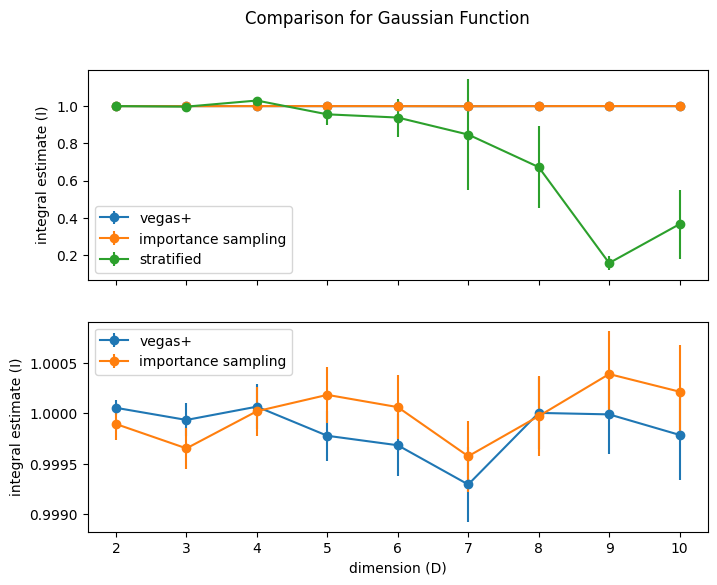
\includegraphics[width=\columnwidth]{../plots/gauss_dimensions.png}
					%height=4cm,width=6cm
				\caption{Comparison of  Gaussian integral estimate $I$ from 50 iterations with 12000 samples after a warmup of 5 iterations with 1000 samples. }
			\end{figure}
		\end{column}
	\begin{column}{0.5 \textwidth}
		\begin{figure}
		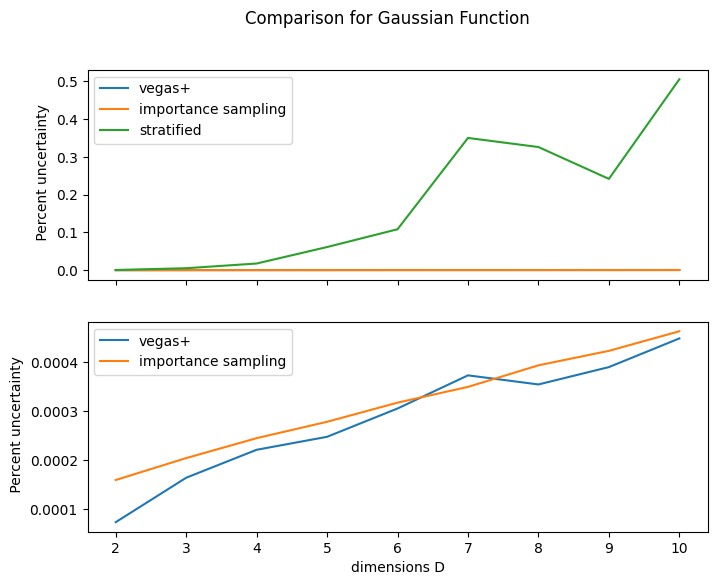
\includegraphics[width=\columnwidth]{../plots/gauss_dims_2.png}
		%height=4cm,width=6cm
		\caption{Comparison of  percent uncertainty of Gaussian integral  from 50 iterations with 12000 samples after a warmup of 5 iterations with 1000 samples. }
		\end{figure}
		\end{column}
	\end{columns}
\end{frame}

\begin{frame}{Dimensional comparison}
	\vspace{-0.5cm}
	\tiny
		\begin{figure}
				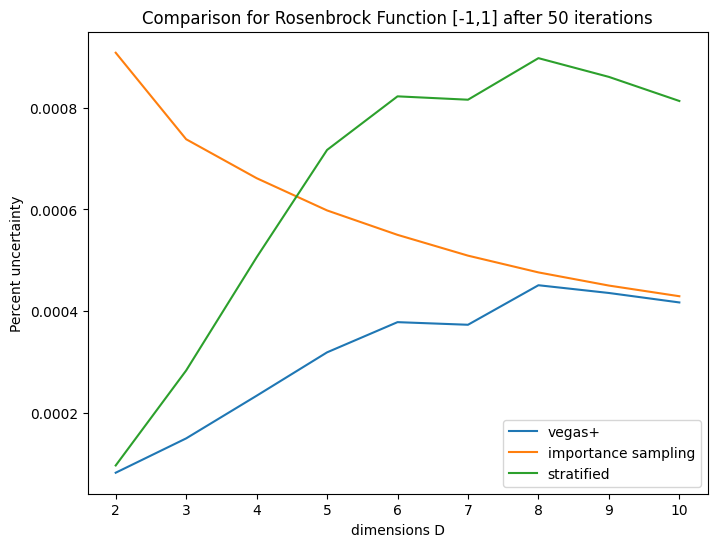
\includegraphics[width=height=4cm,width=6cm]{../plots/rosen_dims_final.png}
				%height=4cm,width=6cm
				\caption{Comparison of  percent uncertainty of Rosenbrock integral  from 50 iterations with 12000 samples after a warmup of 5 iterations with 1000 samples.}
	\end{figure}
		
\end{frame}

\begin{frame}{Gaussian samples comparison}
	\vspace{-0.5cm}
	\tiny
\begin{columns}[T]
	\begin{column}[T]{0.5 \textwidth}
		\begin{figure}
			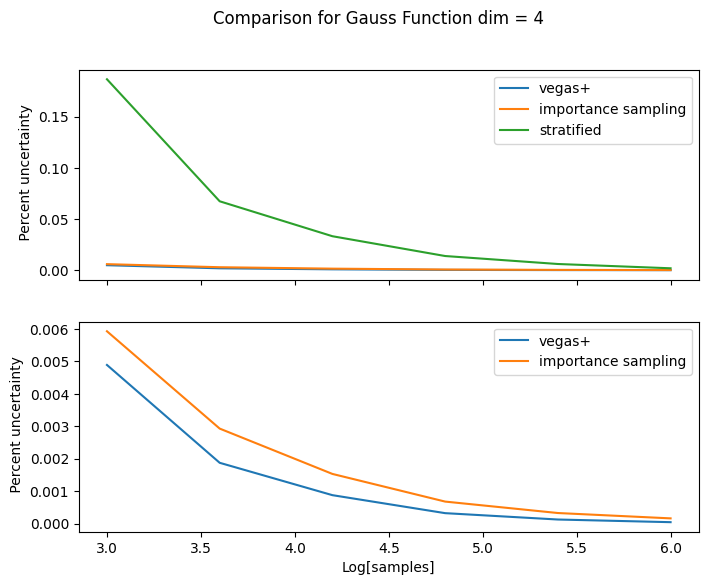
\includegraphics[width=\columnwidth]{../plots/gauss_samples_symm_dim4_log.png}
			%height=4cm,width=6cm
			\caption{Comparison of  percent uncertainty 4-d-Gaussian integralfrom 10 iterations with different samples per iteration after a warmup of 5 iterations with 1000 samples.}
		\end{figure}
	\end{column}
	\begin{column}{0.5 \textwidth}
		\begin{figure}
			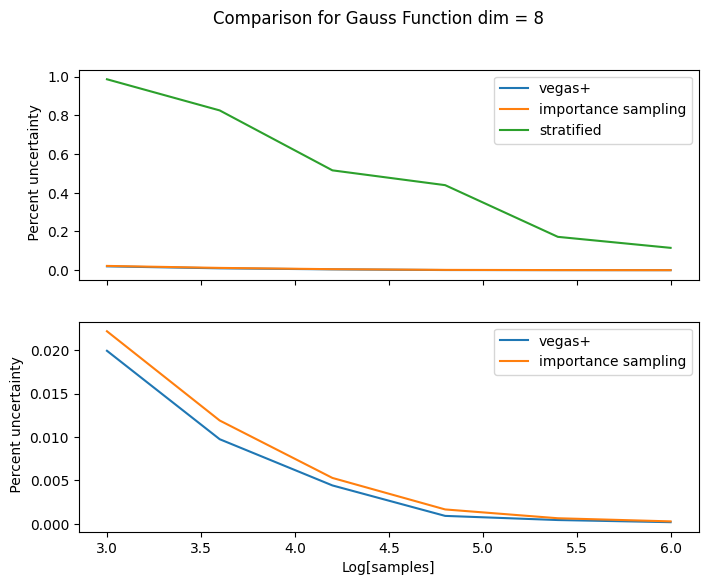
\includegraphics[width=\columnwidth]{../plots/gauss_samples_symm_dim8_log.png}
			%height=4cm,width=6cm
			\caption{Comparison of  percent uncertainty of  8-d-Gaussian integral from 10 iterations with different samples per iteration after a warmup of 5 iterations with 1000 samples.}
		\end{figure}
	\end{column}
\end{columns}
	
\end{frame}

\begin{frame}{Rosenbrock samples comparison}
	\vspace{-0.5cm}
	\tiny
	\begin{columns}[T]
		\begin{column}[T]{0.5 \textwidth}
			\begin{figure}
				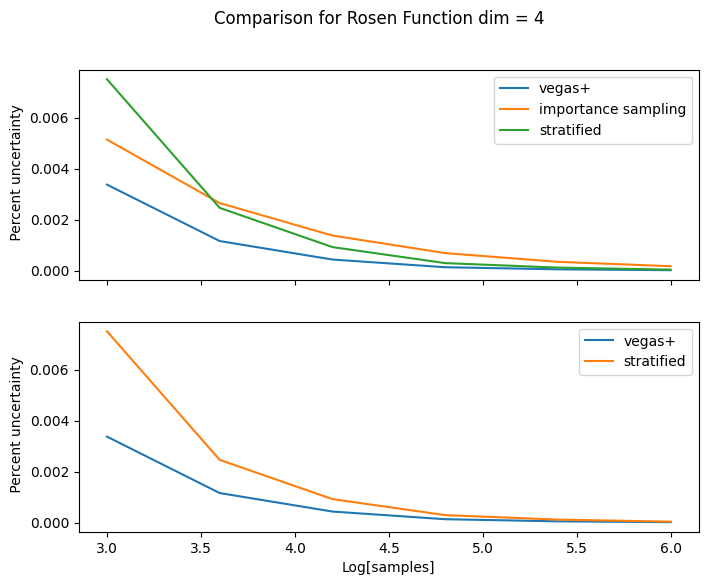
\includegraphics[width=\columnwidth]{../plots/rosen_samples_symm_dim4_log.png}
				%height=4cm,width=6cm
				\caption{Comparison of  percent uncertainty of  4-d-Rosenbrock integral from 10 iterations with different samples per iteration after a warmup of 5 iterations with 1000 samples.}
			\end{figure}
		\end{column}
		\begin{column}{0.5 \textwidth}
			\begin{figure}
				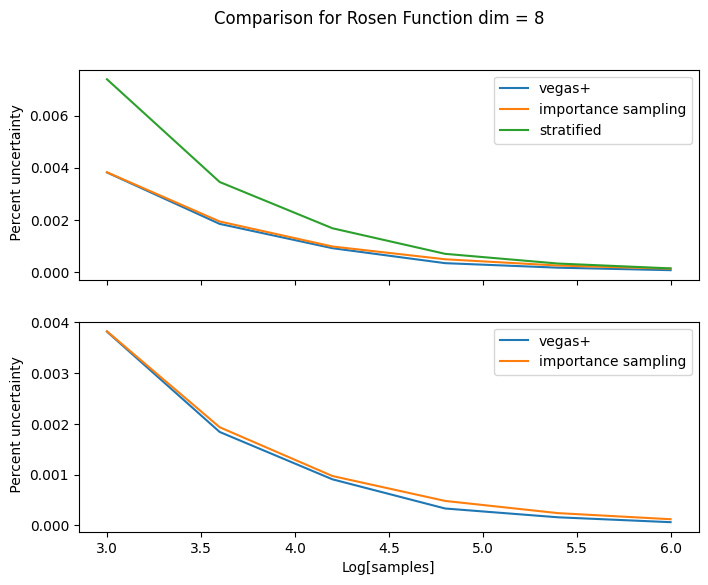
\includegraphics[width=\columnwidth]{../plots/rosen_samples_symm_dim8_log.png}
				%height=4cm,width=6cm
				\caption{Comparison of  percent uncertainty of  8-d-Rosenbrock integral from 10 iterations with different samples per iteration after a warmup of 5 iterations with 1000 samples.}
			\end{figure}
		\end{column}
	\end{columns}
	
\end{frame}

\begin{frame}
	\tiny
	\begin{figure}
		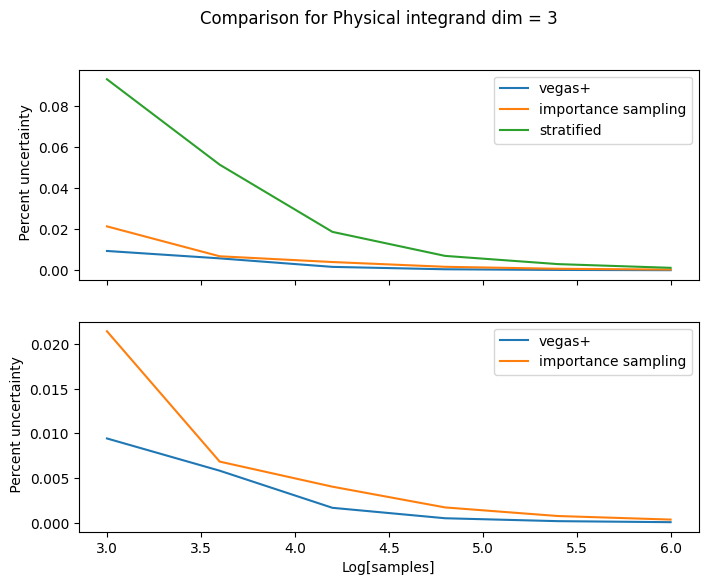
\includegraphics[width=height=4cm,width=6cm]{../plots/dy_aa_samples_log.png}
		%height=4cm,width=6cm
		\caption{Comparison of  percent uncertainty of  3-d physical integral from 10 iterations with different samples per iteration after a warmup of 5 iterations with 1000 samples.}
	\end{figure}
	
\end{frame}

\begin{frame}{Gauss 4-d performance comparison}
	\tiny
	\vspace{-0.4cm}
	\begin{figure}
		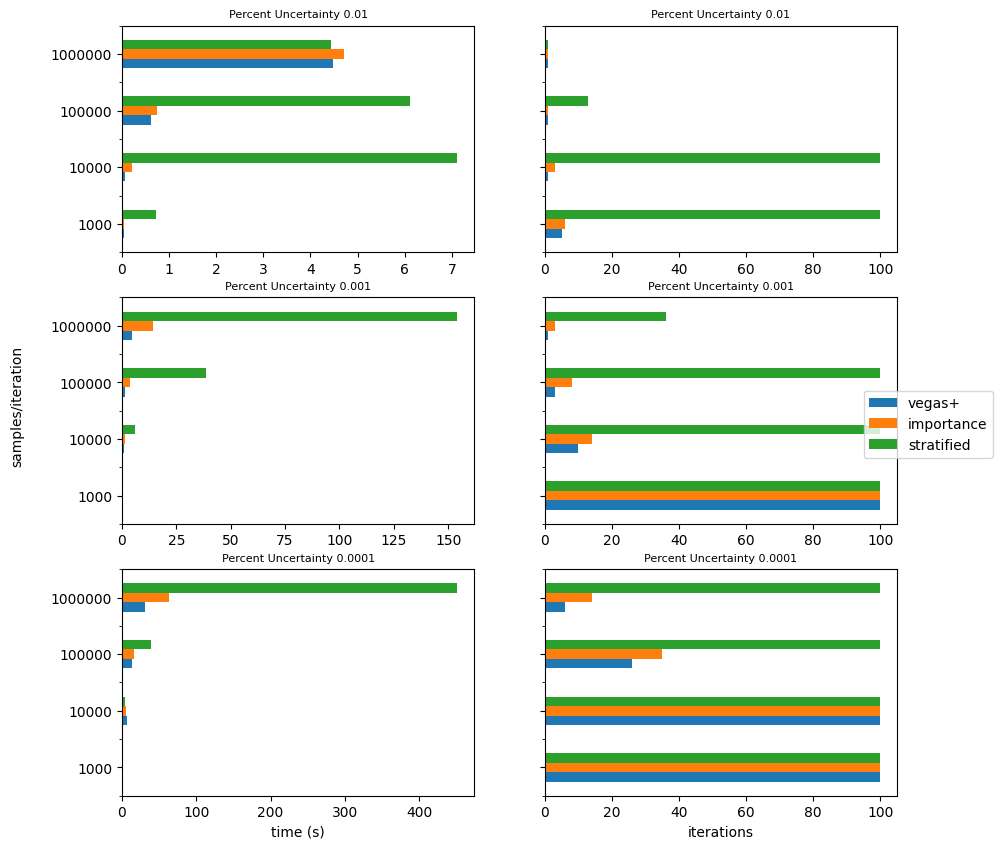
\includegraphics[height=6cm,width=9cm]{../performance_plots/gauss4-d.png}
		%height=4cm,width=6cm
		\caption{Comparison of perfomances between different integration methods at fixed percent uncertainty ( $10^{-2}$, $10^{-3}$ or $10^{-4}$) and at fixed samples per iteration ($10^3$,$10^4$,$10^5$ or $10^6$ ) with $100$ maximum iterations.}
	\end{figure}
	
\end{frame}

\begin{frame}{Gauss 4-d performance comparison}
	\tiny
	\vspace{-0.4cm}
	\begin{figure}
		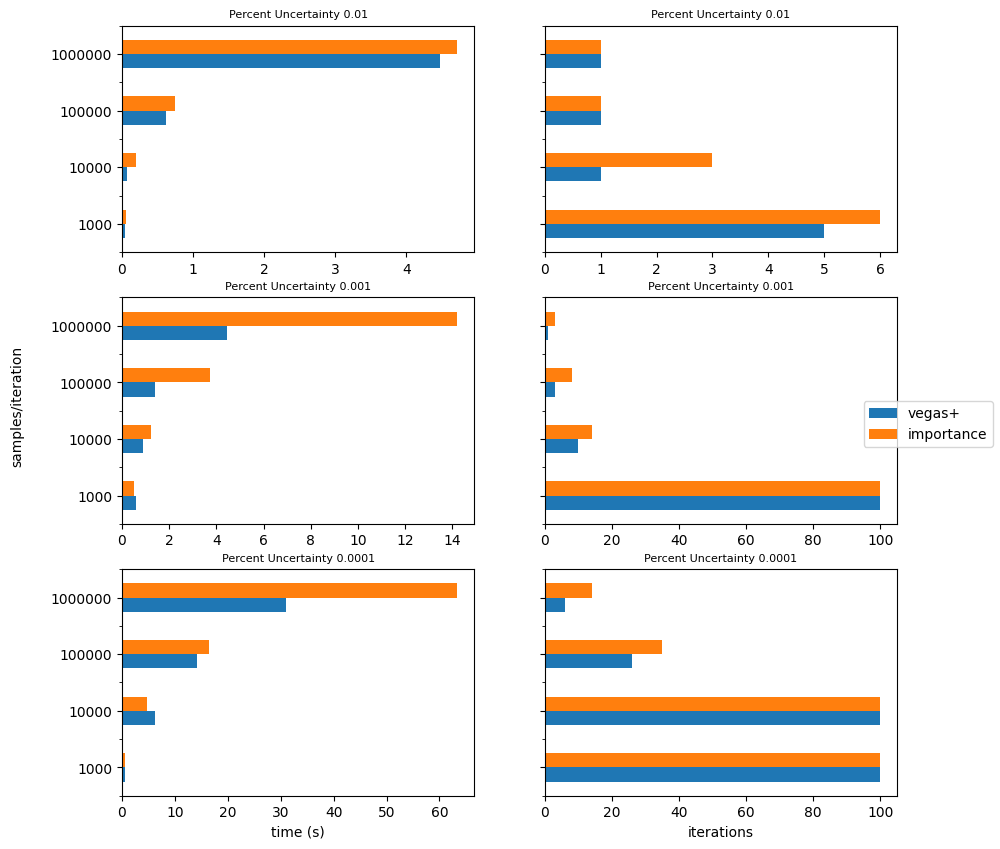
\includegraphics[height=6cm,width=9cm]{../performance_plots/gauss4-d_no_stratified.png}
		%height=4cm,width=6cm
		\caption{Comparison of perfomances between different integration methods at fixed percent uncertainty ( $10^{-2}$, $10^{-3}$ or $10^{-4}$) and at fixed samples per iteration ($10^3$,$10^4$,$10^5$ or $10^6$ ) with $100$ maximum iterations.}
	\end{figure}
	
\end{frame}

\begin{frame}{Gauss 8-d performance comparison}
	\tiny
	\vspace{-0.4cm}
	\begin{figure}
		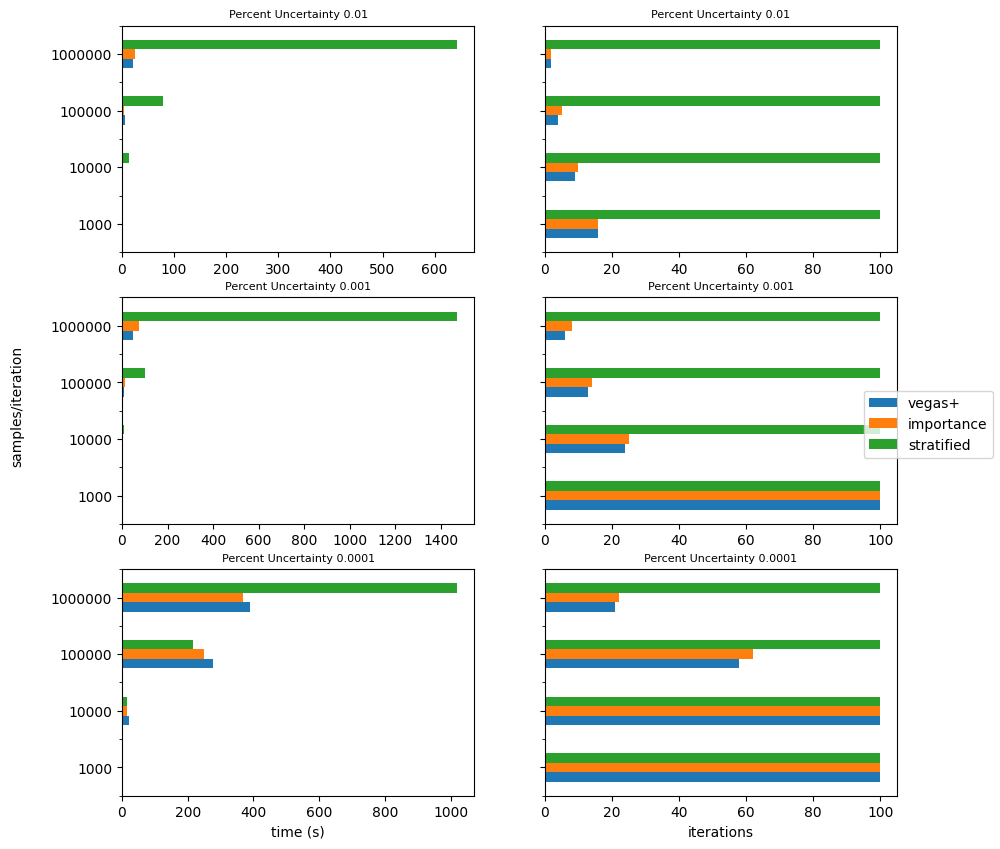
\includegraphics[height=6cm,width=9cm]{../performance_plots/gauss8-d.png}
		%height=4cm,width=6cm
		\caption{Comparison of perfomances between different integration methods at fixed percent uncertainty ( $10^{-2}$, $10^{-3}$ or $10^{-4}$) and at fixed samples per iteration ($10^3$,$10^4$,$10^5$ or $10^6$ ) with $100$ maximum iterations.}
	\end{figure}
	
\end{frame}

\begin{frame}{Gauss 8-d performance comparison}
	\tiny
	\vspace{-0.4cm}
	\begin{figure}
		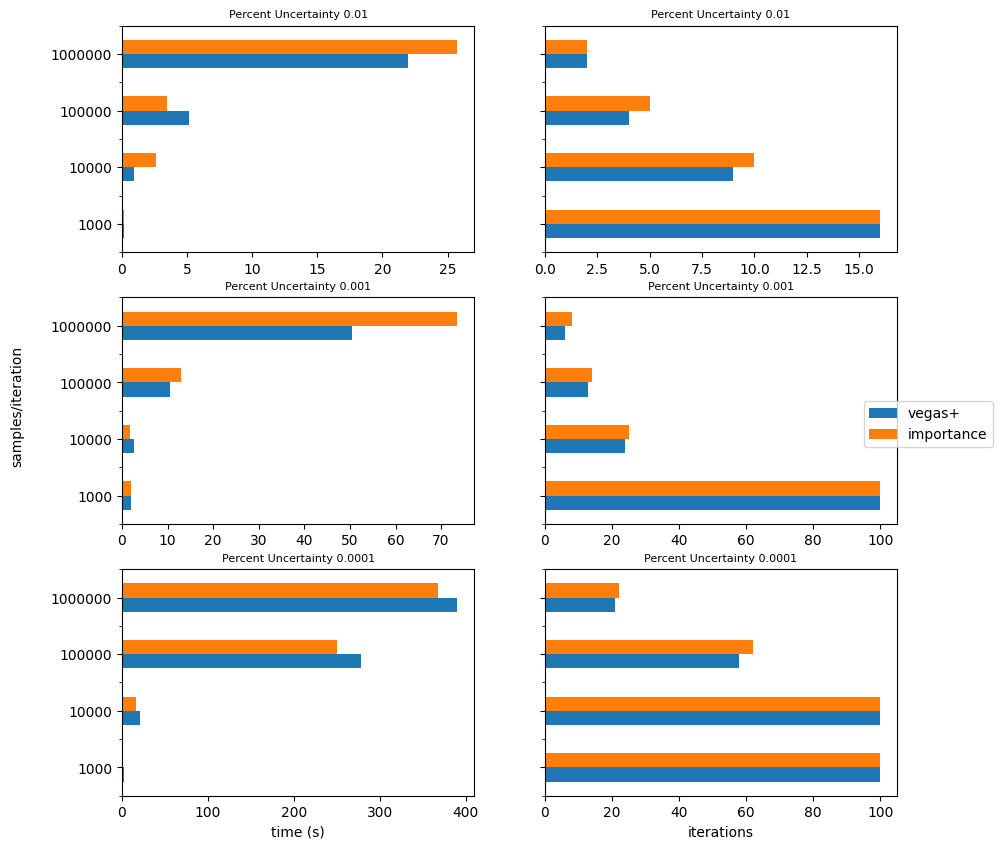
\includegraphics[height=6cm,width=9cm]{../performance_plots/gauss8-d_no_stratified.png}
		%height=4cm,width=6cm
		\caption{Comparison of perfomances between different integration methods at fixed percent uncertainty ( $10^{-2}$, $10^{-3}$ or $10^{-4}$) and at fixed samples per iteration ($10^3$,$10^4$,$10^5$ or $10^6$ ) with $100$ maximum iterations.}
	\end{figure}
	
\end{frame}

\begin{frame}{Rosen 4-d performance comparison}
	\tiny
	\vspace{-0.4cm}
	\begin{figure}
		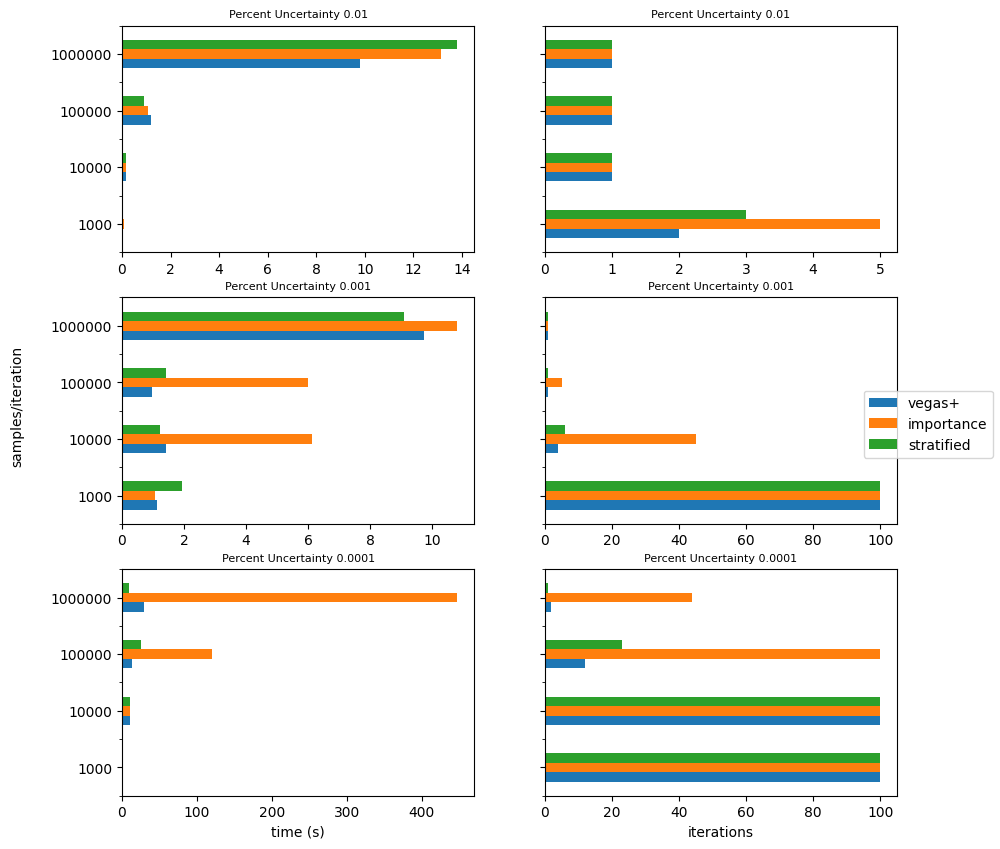
\includegraphics[height=6cm,width=9cm]{../performance_plots/rosen4-d.png}
		%height=4cm,width=6cm
		\caption{Comparison of perfomances between different integration methods at fixed percent uncertainty ( $10^{-2}$, $10^{-3}$ or $10^{-4}$) and at fixed samples per iteration ($10^3$,$10^4$,$10^5$ or $10^6$ ) with $100$ maximum iterations.}
	\end{figure}
	
\end{frame}

\begin{frame}{Rosen 4-d performance comparison}
	\tiny
	\vspace{-0.4cm}
	\begin{figure}
		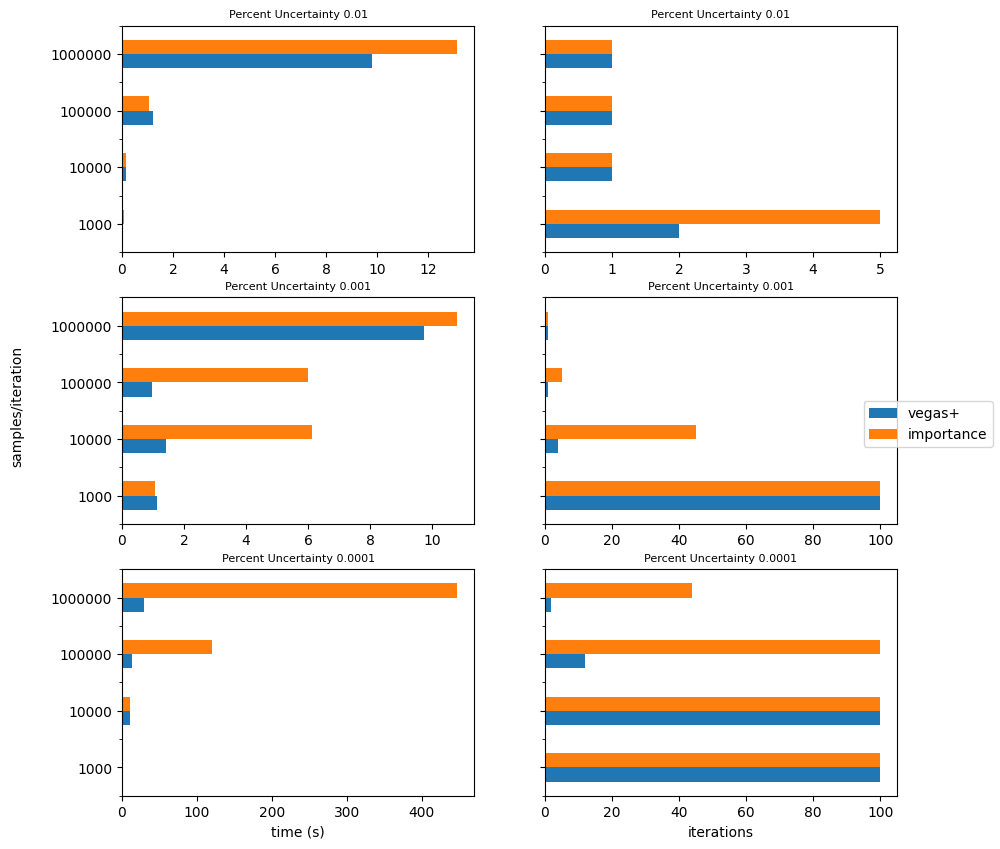
\includegraphics[height=6cm,width=9cm]{../performance_plots/rosen4-d_no_stratified.png}
		%height=4cm,width=6cm
		\caption{Comparison of perfomances between different integration methods at fixed percent uncertainty ( $10^{-2}$, $10^{-3}$ or $10^{-4}$) and at fixed samples per iteration ($10^3$,$10^4$,$10^5$ or $10^6$ ) with $100$ maximum iterations.}
	\end{figure}
	
\end{frame}

\begin{frame}{Rosen 8-d performance comparison}
	\tiny
	\vspace{-0.4cm}
	\begin{figure}
		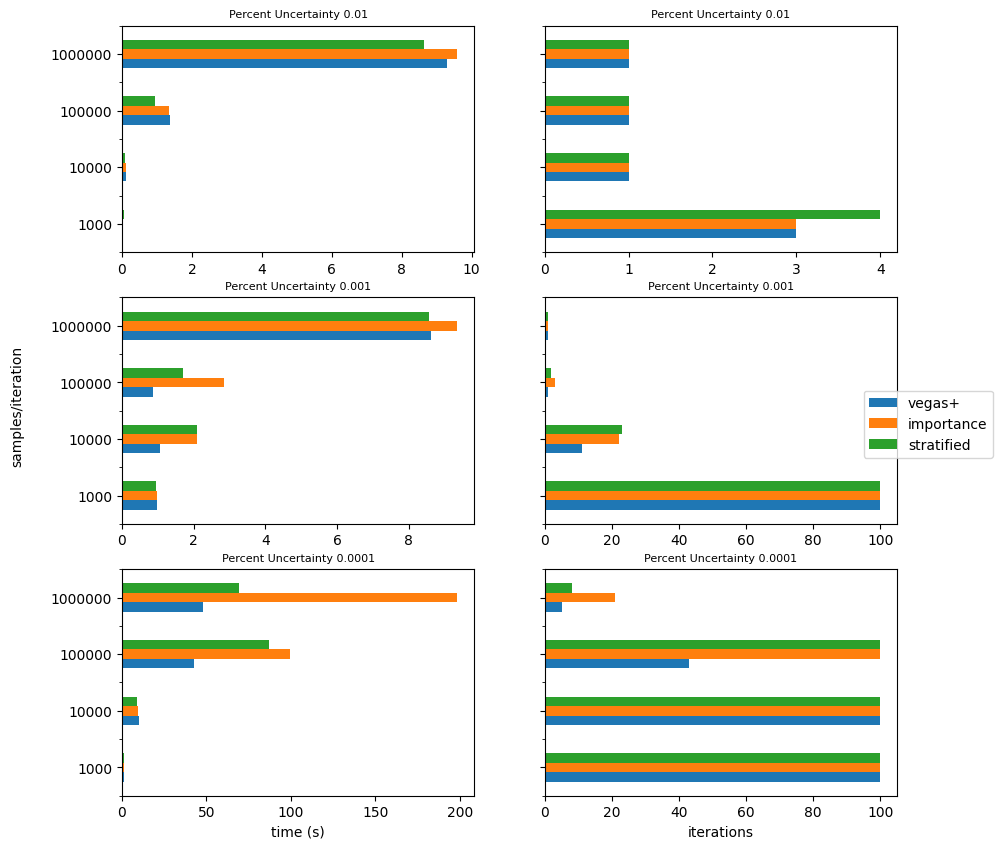
\includegraphics[height=6cm,width=9cm]{../performance_plots/rosen8-d.png}
		%height=4cm,width=6cm
		\caption{Comparison of perfomances between different integration methods at fixed percent uncertainty ( $10^{-2}$, $10^{-3}$ or $10^{-4}$) and at fixed samples per iteration ($10^3$,$10^4$,$10^5$ or $10^6$ ) with $100$ maximum iterations.}
	\end{figure}
	
\end{frame}

\begin{frame}{Rosen 8-d performance comparison}
	\tiny
	\vspace{-0.4cm}
	\begin{figure}
		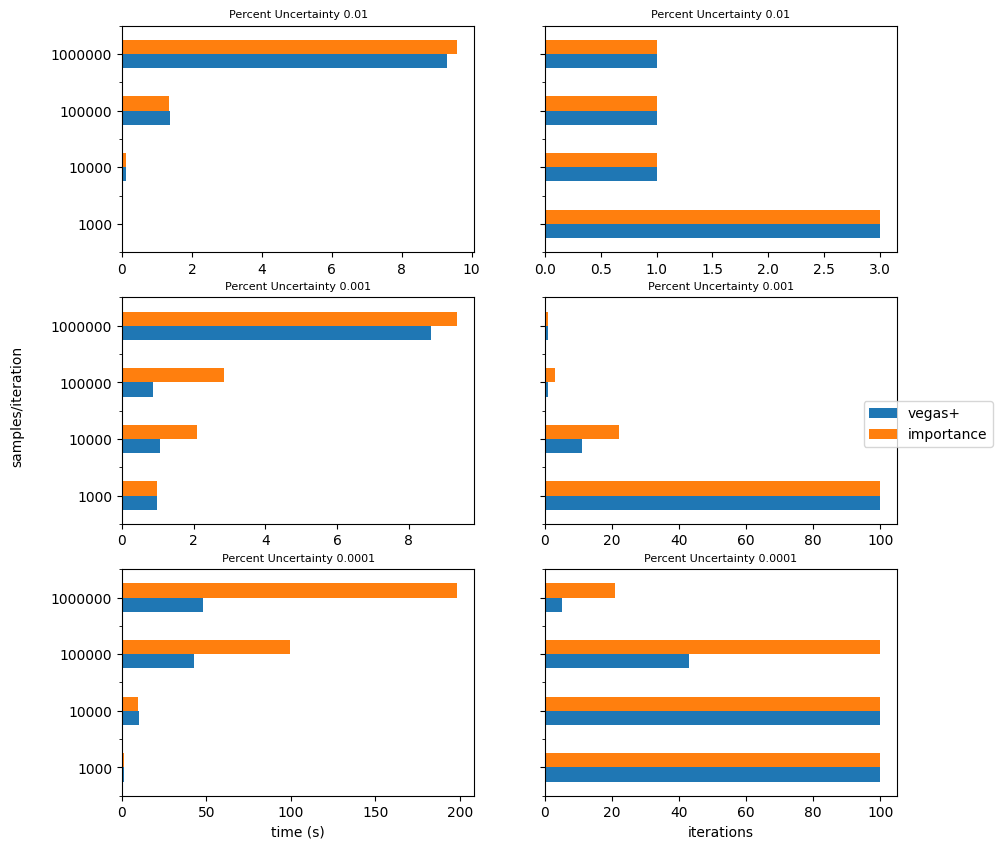
\includegraphics[height=6cm,width=9cm]{../performance_plots/rosen8-d_no_stratified.png}
		%height=4cm,width=6cm
		\caption{Comparison of perfomances between different integration methods at fixed percent uncertainty ( $10^{-2}$, $10^{-3}$ or $10^{-4}$) and at fixed samples per iteration ($10^3$,$10^4$,$10^5$ or $10^6$ ) with $100$ maximum iterations.}
	\end{figure}
	
\end{frame}

\begin{frame}{Physical Integrand performance comparison}
	\tiny
	\vspace{-0.4cm}
	\begin{figure}
		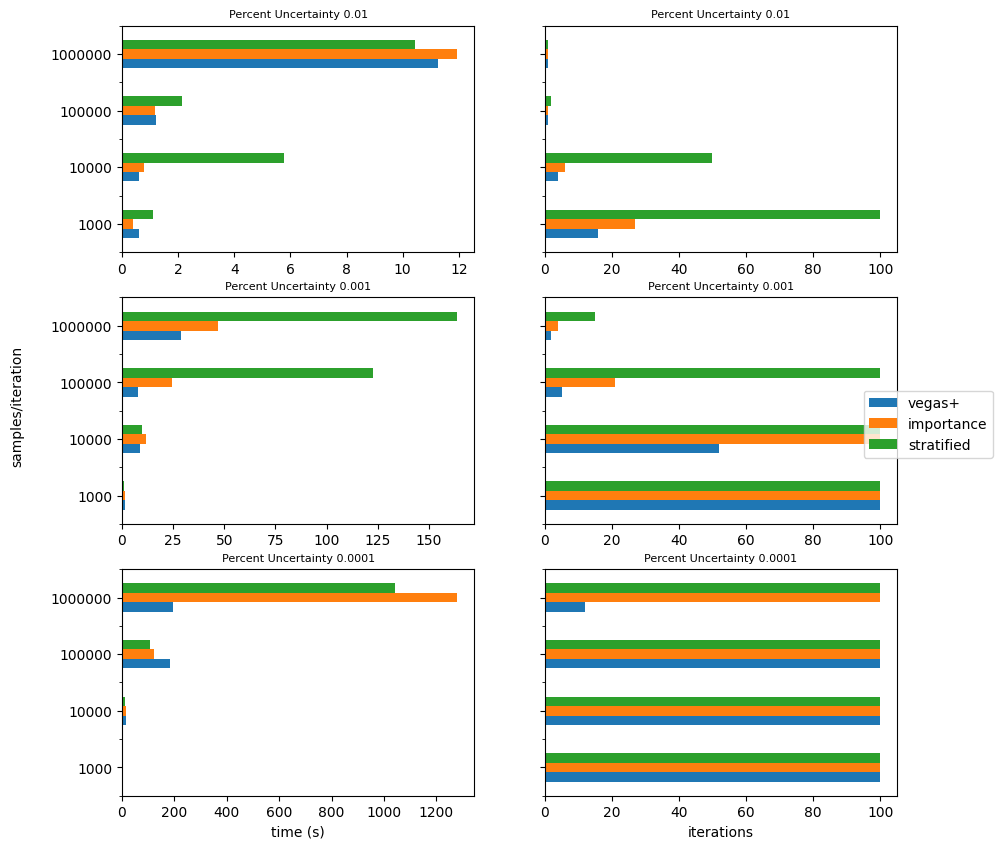
\includegraphics[height=6cm,width=9cm]{../performance_plots/dy_aa.png}
		%height=4cm,width=6cm
		\caption{Comparison of perfomances between different integration methods at fixed percent uncertainty ( $10^{-2}$, $10^{-3}$ or $10^{-4}$) and at fixed samples per iteration ($10^3$,$10^4$,$10^5$ or $10^6$ ) with $100$ maximum iterations.}
	\end{figure}
	
\end{frame}

\begin{frame}{Physical Integrand performance comparison}
	\tiny
	\vspace{-0.4cm}
	\begin{figure}
		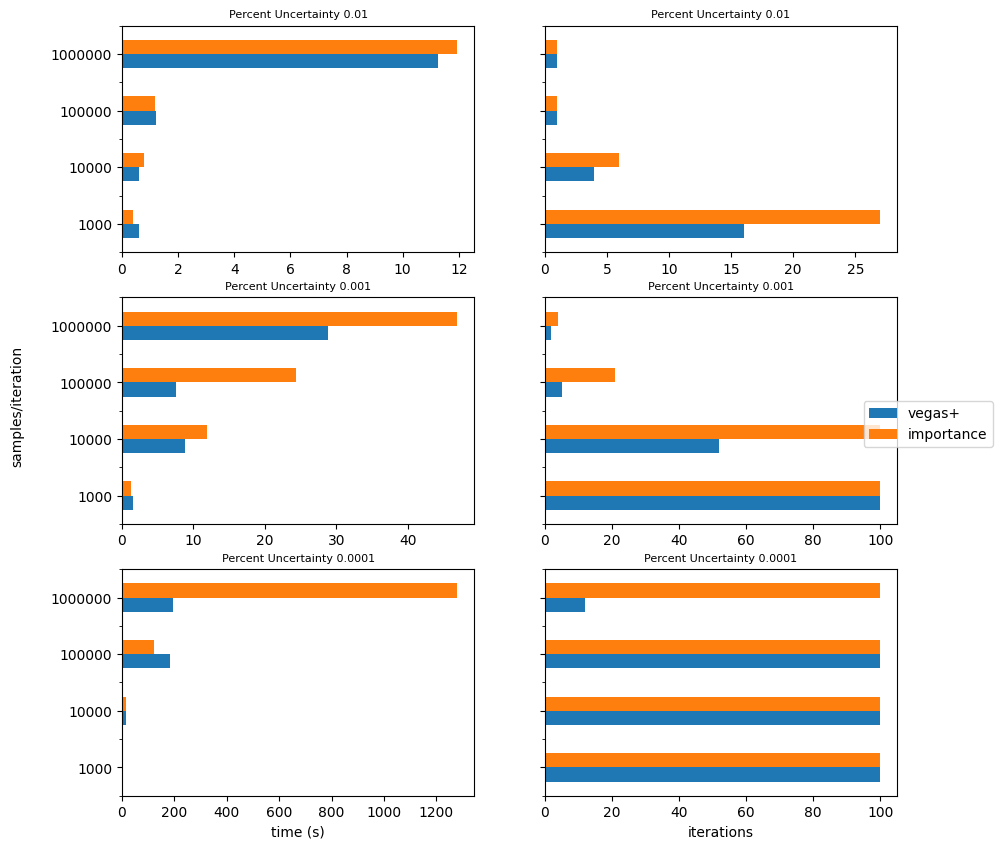
\includegraphics[height=6cm,width=9cm]{../performance_plots/dy_aa_no_stratified.png}
		%height=4cm,width=6cm
		\caption{Comparison of perfomances between different integration methods at fixed percent uncertainty ( $10^{-2}$, $10^{-3}$ or $10^{-4}$) and at fixed samples per iteration ($10^3$,$10^4$,$10^5$ or $10^6$ ) with $100$ maximum iterations.}
	\end{figure}
	
\end{frame}


\end{document}